\chapter{Introduction}
\label{intro}

\section{Volumetric effects}

\begin{figure}
	\centering
	\subfloat[Clouds]{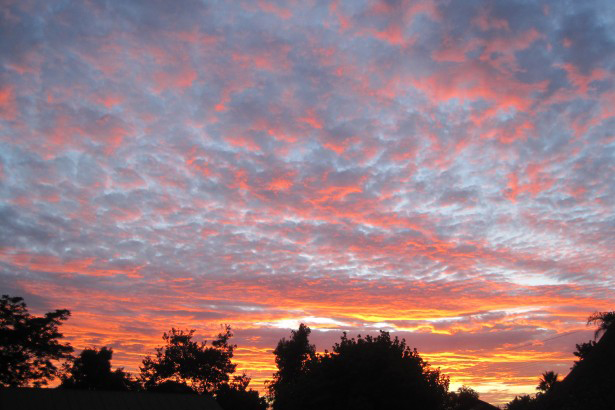
\includegraphics[width= 2in]{clouds.jpg}}
	~
	\subfloat[A water droplet]{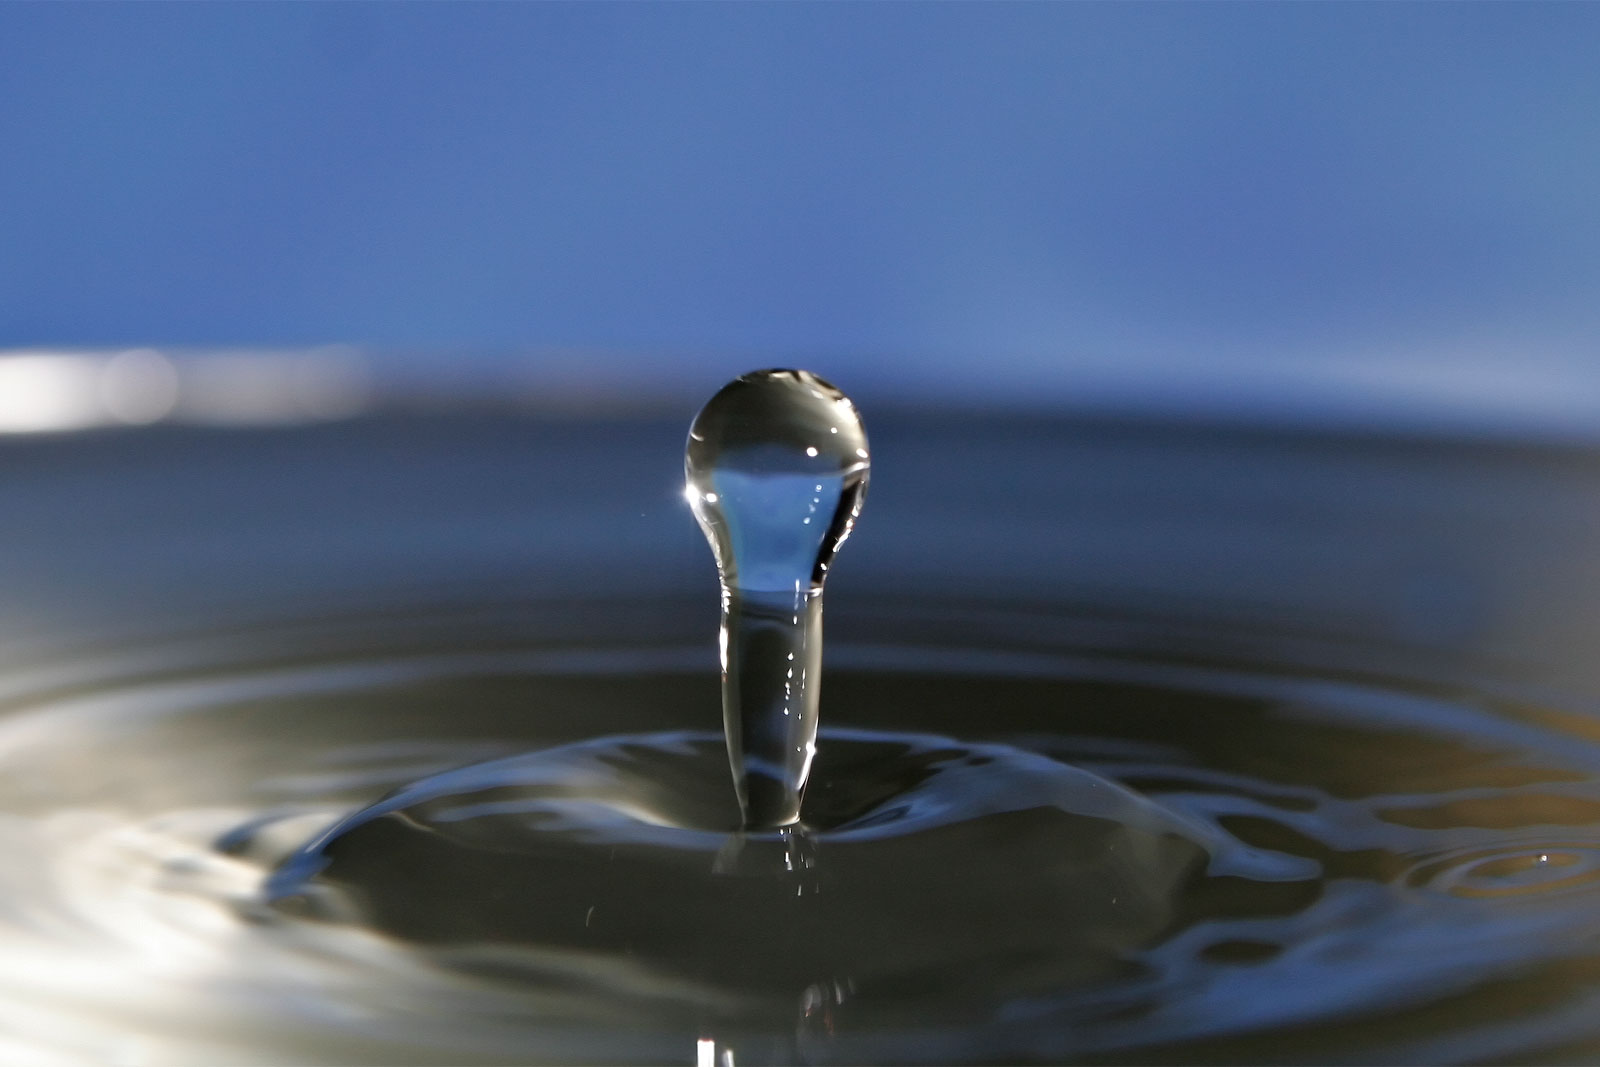
\includegraphics[width= 2in]{water_droplets.jpg}}

	\caption{The lighting of clouds and water droplets is volumetric in nature}
	\label{fig:volumetric-effects}
\end{figure}

Many effects in the real world are volumetric in nature, such as fluids, clouds, fire, fog, and dust. A volumetric effect is one for which the inner volume has an influence on the lighting of an object, rather than just its surface. These effects are highly sought after in video games, but existing solutions often do not model them volumetrically, instead utilising crude approximations. Despite being fast to render using existing hardware, it is difficult to produce realistic results with these approaches.

\begin{figure}
\centering
	\subfloat[A naked flame]{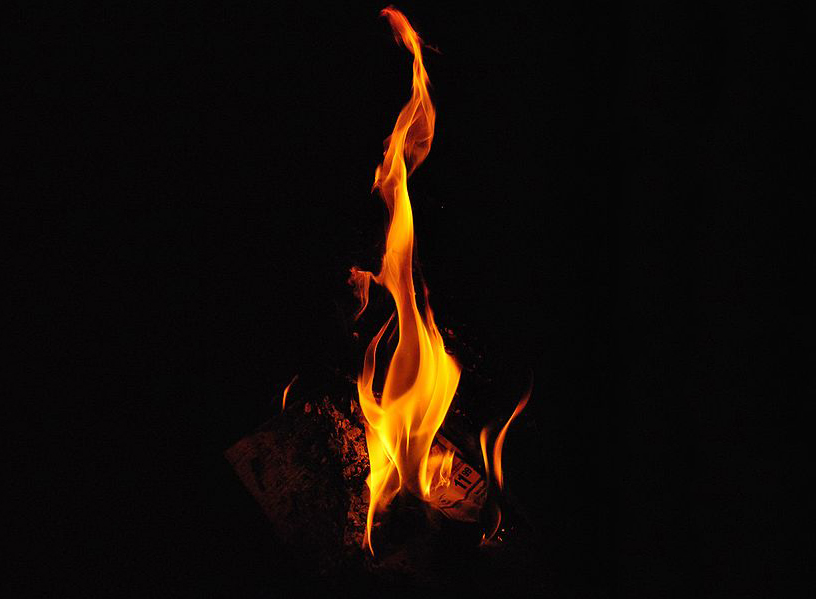
\includegraphics[width= 2in]{fire.jpg}}
	~
	\subfloat[Dust]{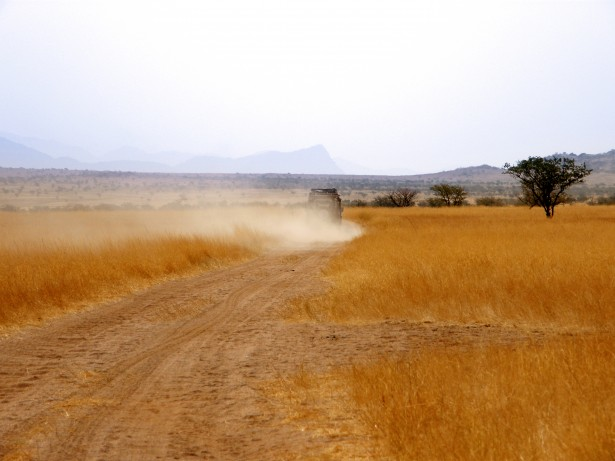
\includegraphics[width= 2in]{dust.jpg}}

	\caption{Other effects which must be considered volumetrically to be rendered physically are fire and dust}
	\label{fig:fire_dust-effects}
\end{figure}

To produce truly realistic volumetric effects, it would be ideal to model the volumes that cause them, and then be able to render them directly. Unfortunately, this is not a trivial problem to solve, especially in modern 3D hardware which is focused on rendering geometry rather than volumes.

Take for example clouds. In the real world, the lighting of clouds is not caused by the way that light hits a surface. Perhaps the most important factor that results in the appearance of clouds is the scattering of light as sunlight hits the atmospheric particles that make up the cloud. As light is scattered in many directions, including inside the cloud, it becomes important to consider the inner volume of the cloud rather than the geometry that describes its shape.

In order to understand the problems involved in rendering volumetric effects on 3D rendering hardware, it is important to understand the mechanism by which 3D rendering is accomplished on this hardware: rasterisation.

\section{Rasterisation}
Rasterisation is currently the most popular rendering algorithm for generating three-dimensional images in video games. It is also the purpose for which modern graphics processing hardware is heavily specialised.

The basic mechanism by which rasterisation functions is converting polygons to a raster image, a rectangular grid of pixels with each pixel having a defined colour. Typically, triangles are utilised, as any geometric shape, whether convex or concave, can be easily triangulated. Graphics hardware then has the simple job of processing these triangles to produce a raster image.

\subsection{Polygon scan conversion}
\label{pct}
A common method of accomplishing rasterisation is polygon scan conversion. By considering a single scan-line of a polygon at a time, identifying the edges, and filling in the scan-line in between them, a raster image of the polygon can be created. As in figure \ref{fig:tri-edges}, this is trivial for a convex polygon such as a triangle, as there will only ever be two edges intersecting a scan-line.

\begin{figure}
\centering
	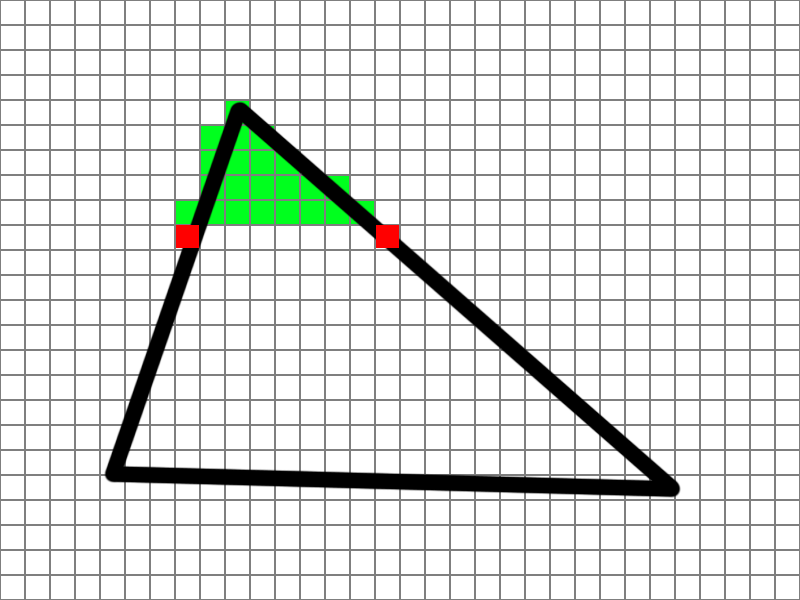
\includegraphics[width=8cm]{tri-edges.png}
	\caption{A triangle being rasterised. Green pixels have already been filled, while red pixels are the edges that have been identified for the current scanline}
	\label{fig:tri-edges}
\end{figure}

Repeating this technique for every scan-line covered by the triangle produces a raster image of the polygon, as shown in figure \ref{fig:rasterised_polygon}.

\begin{figure}
\centering
	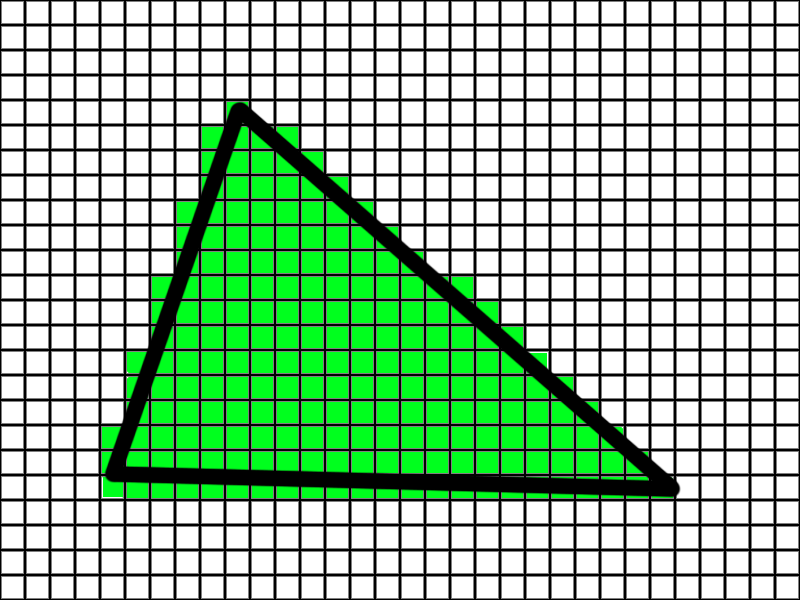
\includegraphics[width=8cm]{rasterised_polygon.png}
	\caption{A polygon that has been rasterised by polygon scan conversion}
	\label{fig:rasterised_polygon}
\end{figure}

\subsection{Extension to 3D graphics}
This technique is then extended to 3D graphics using a projection calculation which maps 3D geometry to a position on the screen. During rasterisation, the pixels can also be shaded using attributes such as the position of the point relative to any lights, and the normal of the plane the point lies on to produce a convincing result as shown in figure \ref{fig:cube_render}.

\begin{figure}
\centering
	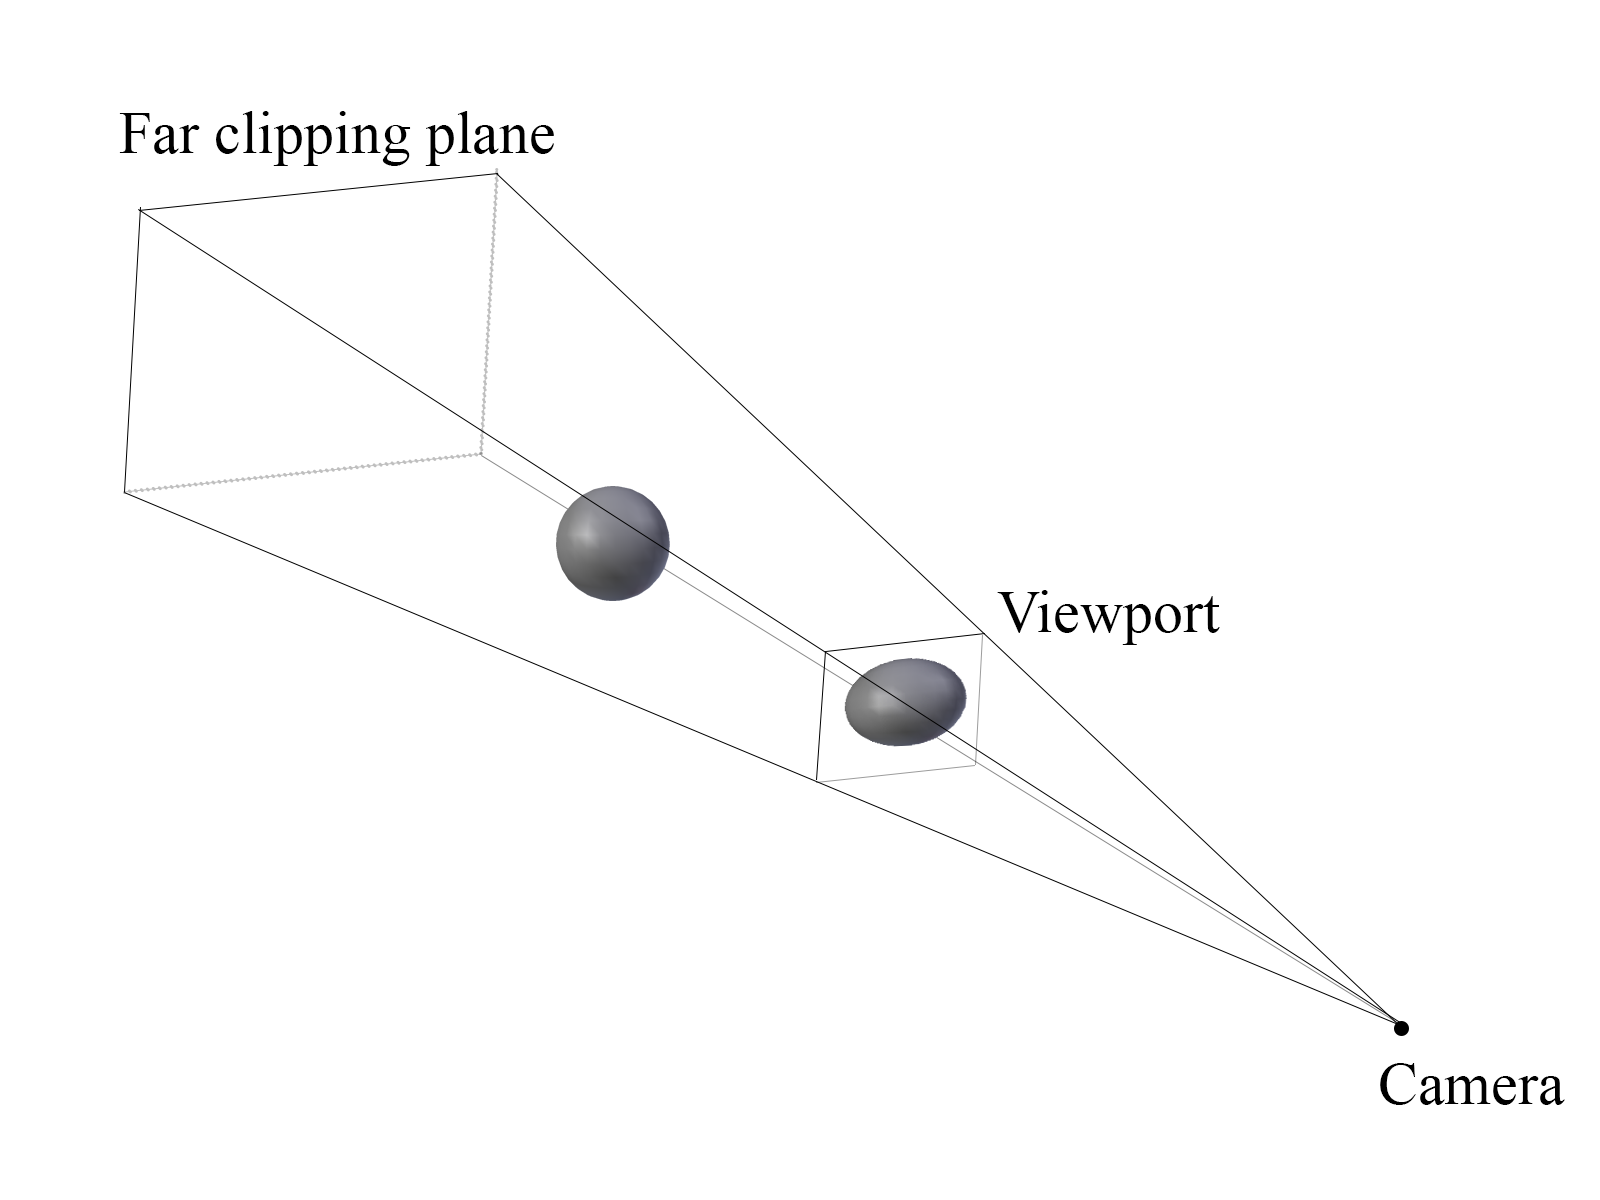
\includegraphics[width=16cm]{frustum.png}
	\caption{An illustration of how 3D objects are mapped to the screen using a perspective projection calculation. A 3D sphere is being rendered to the 2D viewport}
	\label{fig:perspective_calculation}
\end{figure}

\subsection{Triangulation}
Triangulation is the process of dividing a surface into triangles so it can be easily rasterised. Triangles are convex in nature, and so are trivial to rasterise, (see section \ref{pct} on polygon scan conversion.) In addition, any flat geometric surface can be tessellated into triangles, and any curved surface can be reasonably approximated for the purposes of 3D rendering.

Take, for example, a cube mesh. A cuboid is made up of 6 rectangular faces. Each face can then be divided into two triangles.

\begin{figure}
\centering
	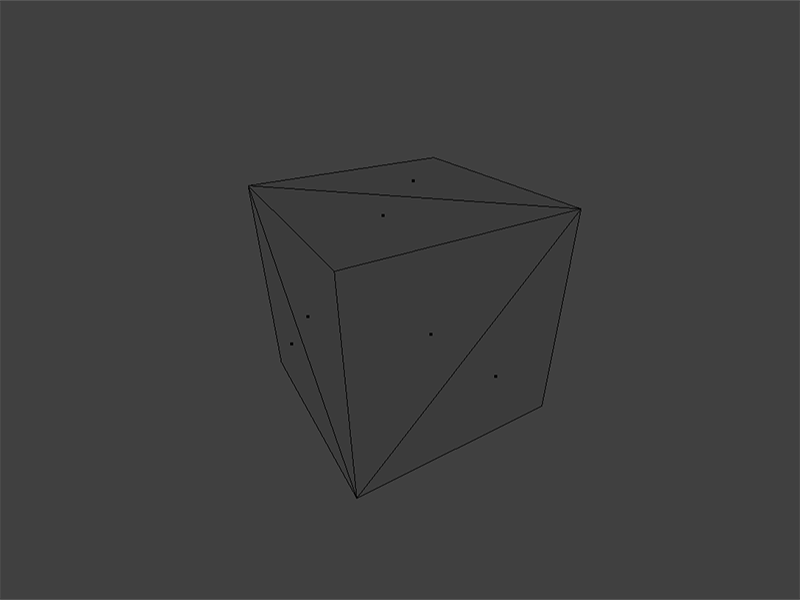
\includegraphics[width=12cm]{cube_triangulation.png}
	\caption{A demonstration of how a cube is triangulated}
	\label{fig:cube_triangulation}
\end{figure}

The vertices of the cube are then transformed using a perspective projection, and the triangles are rasterised using polygon scan conversion.

\begin{figure}
\centering
	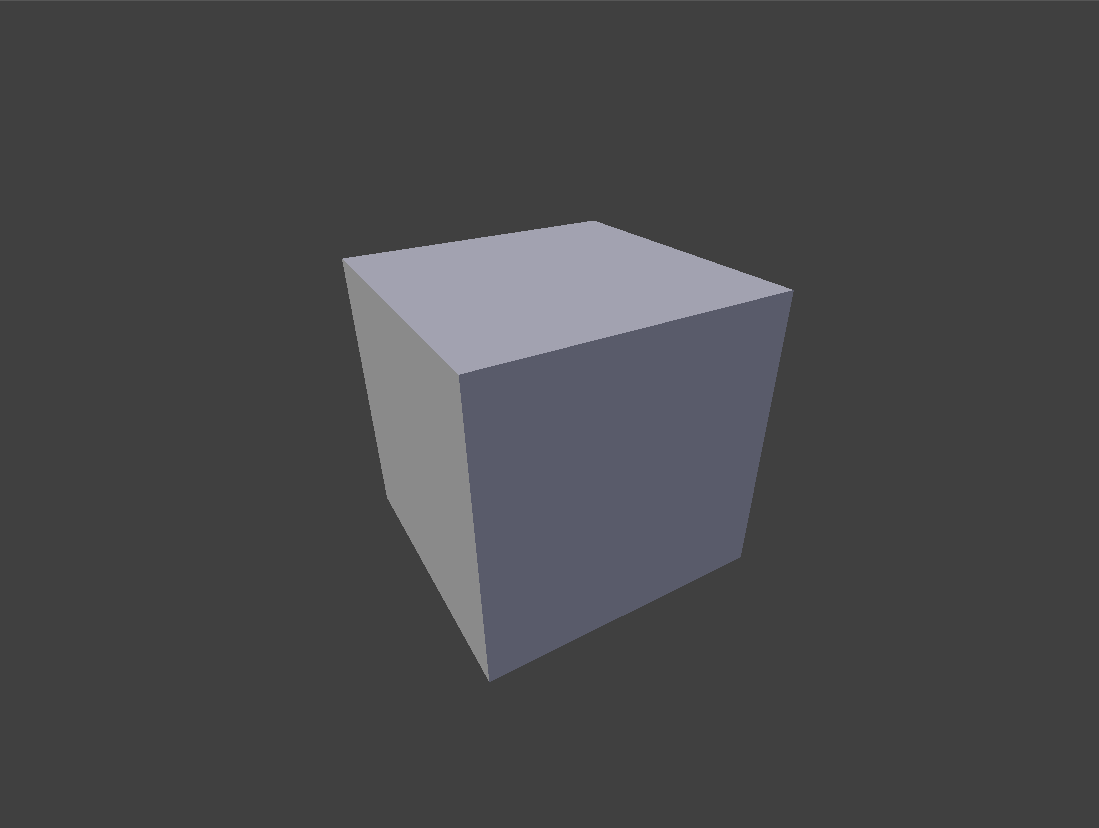
\includegraphics[width=8cm]{cube_rendered.png}
	\caption{The result image once a cube has been rasterised}
	\label{fig:cube_render}
\end{figure}

\subsection{Limitations}
Despite rasterisation producing convincing and, in some applications, even realistic results, it has a number of limitations when it comes to the rendering of volumetric effects.

For the purposes of rendering 3D volumes, the major limitation of rasterisation-based rendering is that it can only consider geometry. Therefore, it only considers the surfaces of objects that are being rendered, and not the volumes bounded within those surfaces. Without considering the inner volume, it becomes very difficult to render these effects realistically, and impossible to render them physically.

Another key limitation of rasterisation is that it only considers reflection, and even then, only an approximation of the light reflected from the current polygon. Only the current polygon is ever considered during rasterisation, making global effects such as reflection and refraction within the scene impossible.

Despite these key limitations, there has been some success in the mapping of volumetric effects to rasterisation hardware.

\subsection{Existing rasterisation-based approaches}

\subsubsection{Skyboxes}
Many games render clouds by mapping a cloud texture onto a sky box or sphere, and then rendering this in the background as shown in figure \ref{fig:skybox}. This structure then surrounds the player, and is typically locked in place relative to the player, such that the player can never get closer to or farther away from it. The sky texture is then projected onto this structure, providing the background imagery for a scene.

\begin{figure}
\centering
	\centering
	\subfloat[]{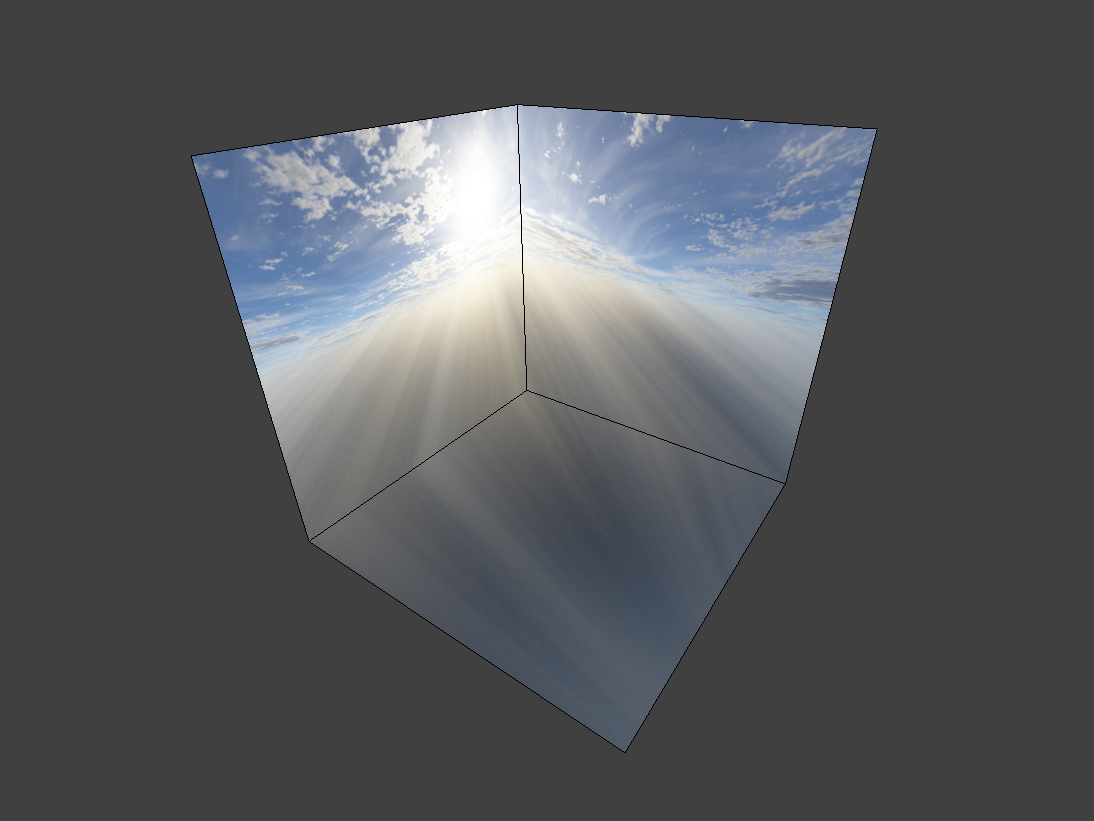
\includegraphics[width= 2in]{skybox.png}}
	~
	\subfloat[]{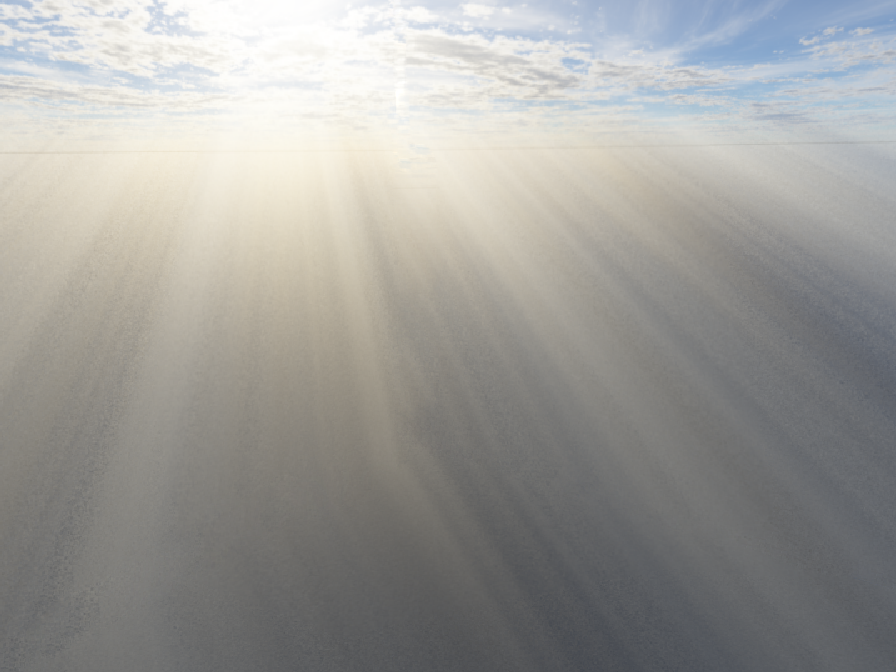
\includegraphics[width= 2in]{skybox_ingame.png}}

	\caption{Mapping of clouds onto a skybox, and the result in-game}
	\label{fig:skybox}
\end{figure}

While this may be sufficient for some applications, for example when clouds are in the distant background, clouds rendered in this manner can never be anything more than 2D images. Take for example a flight simulator. Using this type of software, it would be expected that the user would be able to fly close to, or even inside clouds, but as sky boxes can only ever be background imagery, such techniques are inappropriate for this type of application. Even for games in which the player is not expected to be able to reach the clouds, if the player is sufficiently close enough, the clouds should appear to move relative to each other, due to perspective or due to the effects of weather. Using a texture to represent the sky can not simulate this effect unless multiple layers are used, and even then this approach is extremely limited.

\begin{figure}
\centering
	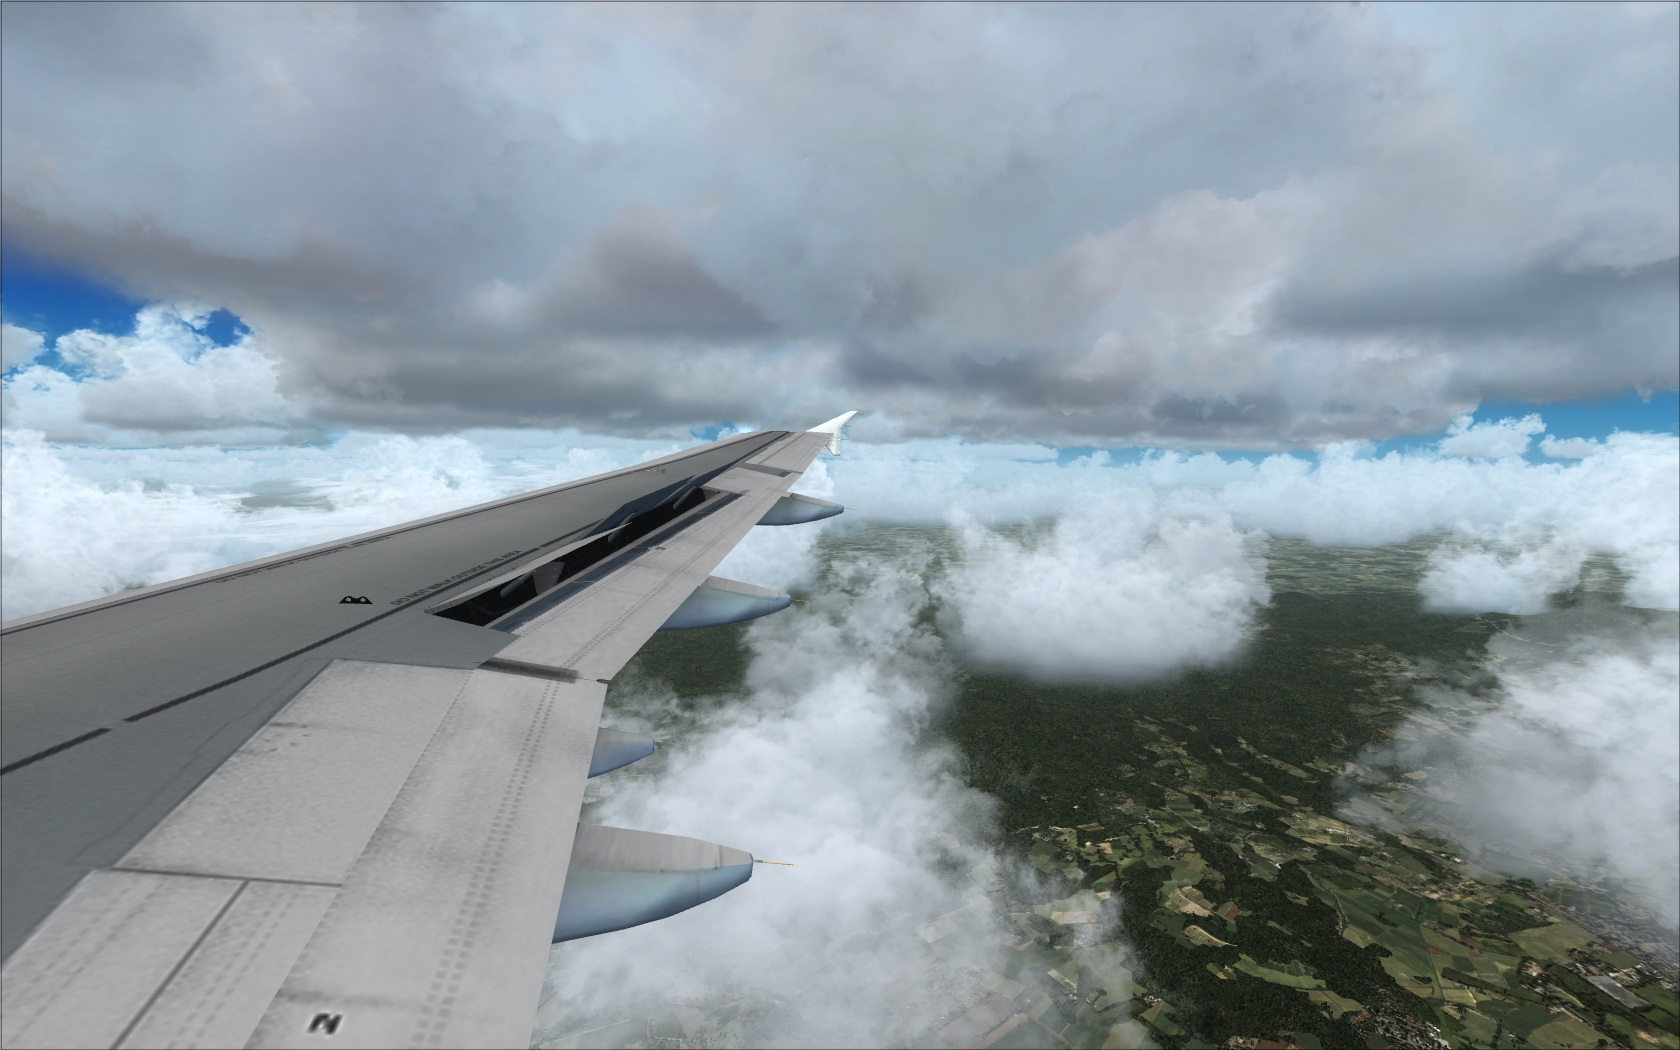
\includegraphics[width=12cm]{flightsim.jpg}
	\caption{Clouds in Microsoft Flight Simulator X}
	\label{fig:flight_sim_clouds}
\end{figure}

\subsubsection{Billboards}
In 3D rendering, billboards are flat, texture-mapped planes that always face the camera. This allows them to appear at different scales and move relatively to each other based on the perspective of the camera. Billboards can be used to efficiently simulate a variety of volumetric structures, by overlapping a number of different images and blending them as appropriate to obtain desired appearance.

\begin{figure}
\centering
	\centering
	\subfloat[]{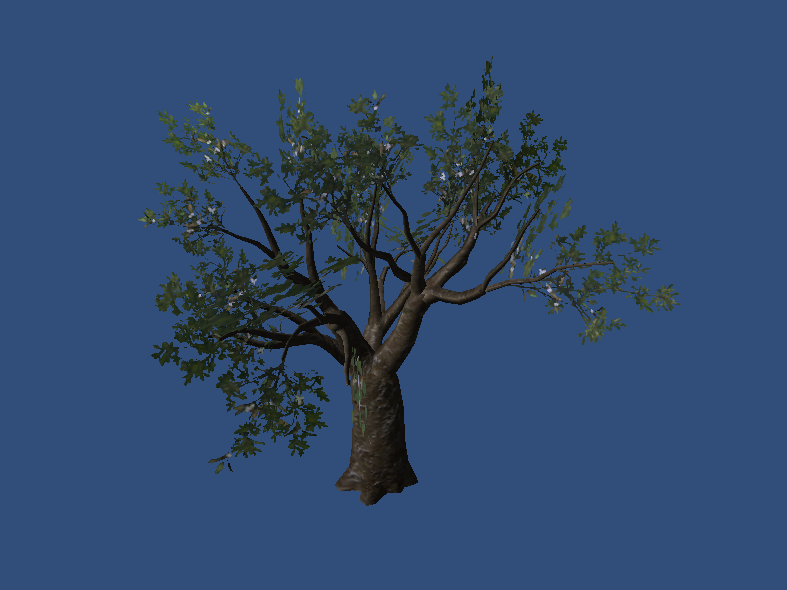
\includegraphics[width=3in]{tree.png}}
	~
	\subfloat[]{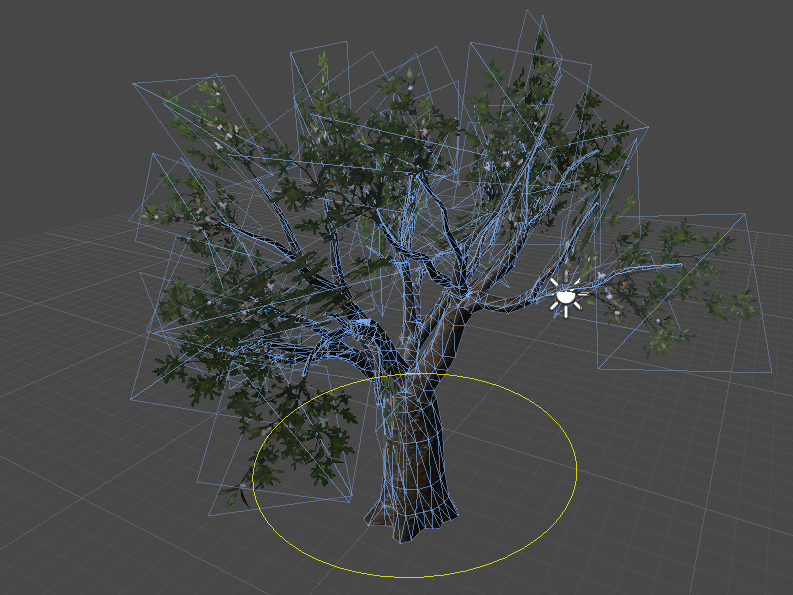
\includegraphics[width=3in]{tree_billboards.png}}

	\caption{Use of texture-mapped quads to simplify a tree mesh. Each quad represents many leaves, greatly reducing the complexity when compared with other representations}
	\label{fig:billboard_tree_quality}
\end{figure}

Billboards have been used effectively to simulate 3D volumetric clouds. \cite{harris02real} simulates the scattering of light within clouds, rendering the result to billboards which are then subtly used to represent the cloud volumes. As the billboards can be reused between multiple frames, this approach allows the realistic, physically based rendering of clouds.

This is a promising approach, and demonstrates the rendering of realistic looking clouds up close and far away as far away clouds can be reused. \citeauthor{harris02real}'s approach, however does not simulate global effects, so still falls short of the objective of simulating true volumetric clouds.

\subsubsection{Marching cubes}
Marching cubes, a technique published in \cite{lorensen87marchingcubes}, is a method of generating polygonal meshes from volumes in order to render them with standard polygon rasterisation hardware. Marching cubes extracts a polygonal approximation of an isosurface, a closed surface that separates the outside of a volume from the inside, defined by an isovalue for which all voxels with greater isovalues are inside the volume and all voxels with lower isovalues are outside.

\begin{figure}
\centering
	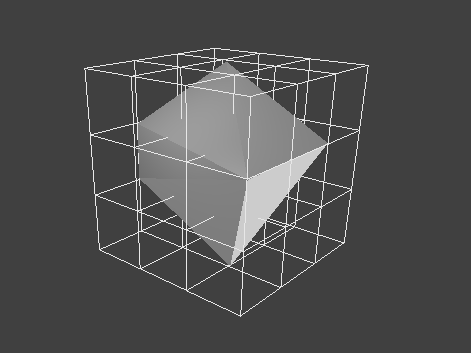
\includegraphics[width=8cm]{gridsampled.png}
	\caption{A volume sampled on a 3D scalar grid. The volume is sampled at the vertices of the grid, and the grid cells are then marched to produce a polygonal approximation of the volume}
	\label{fig:scalar_field_approximation}
\end{figure}

The volume is sampled at each vertex of a regular grid, with each cell defined by its vertices and the isovalue of each vertex, as shown in figure \ref{fig:scalar_field_approximation}. By comparing the isovalue of each vertex against the isovalue of the surface, and therefore determining which vertices lie inside, and which outside the volume, it is possible to create a polygonal approximation of the intersection of the isosurface with the current grid cell. Each grid cell is then considered individually, by "marching" from one cell to the next, in order to create a polygonal approximation of the volume. The detail level of the final mesh depends on the resolution selected for the scalar grid which is used to sample the volume.

The major advantage of this approach is that the resulting polygon mesh maps directly to existing rasterisation hardware, and is therefore as efficient to render as any polygon mesh. However, the major disadvantage for the purposes of volumetric effects is that marching cubes only considers an isosurface, ignoring the inside of the volume and instead focusing on the rendering of the surface, making it inappropriate for considering volumetric effects.

\subsubsection{Texture-based methods}
Texture mapping has also been successfully used to map volume rendering onto rasterisation hardware. \cite{engel02interactivehigh-quality} utilises 3D textures representing slices, each of which represents a view-aligned slice through the volume. Overlapping samples are then composited using hardware alpha blending, in order to create a 3D image of the volume, considering the volume rather than just its surface.

The advantages of this method are that it maps onto traditional graphics hardware very well, resulting in extremely high performance on very common consumer hardware. Unlike approaches which only consider isosurfaces, such as marching cubes, this approach allows us to consider the internals of the volume by means of blending, meaning that it should be possible to model volumetric effects using this approach.

Unfortunately, this approach does not allow us to consider the effects of light that involve reflection, refraction, or scattering, as that would require changes in the direction of light, and this approach can only consider overlapping parts of the volume.

\section{Ray tracing}
Another approach to volume rendering, that does not attempt to map volume rendering problems to rasterisation, is ray tracing. Ray tracing functions by following rays of light backwards from the eye and out into the scene, as shown in figure \ref{fig:ray_casting}. By casting a ray outwards into the scene for each pixel on the screen, and shading that pixel in accordance with the properties of the hit surface, it is possible to produce a 3D image of the scene similar to that produced by means of rasterisation.

\begin{figure}
\centering
	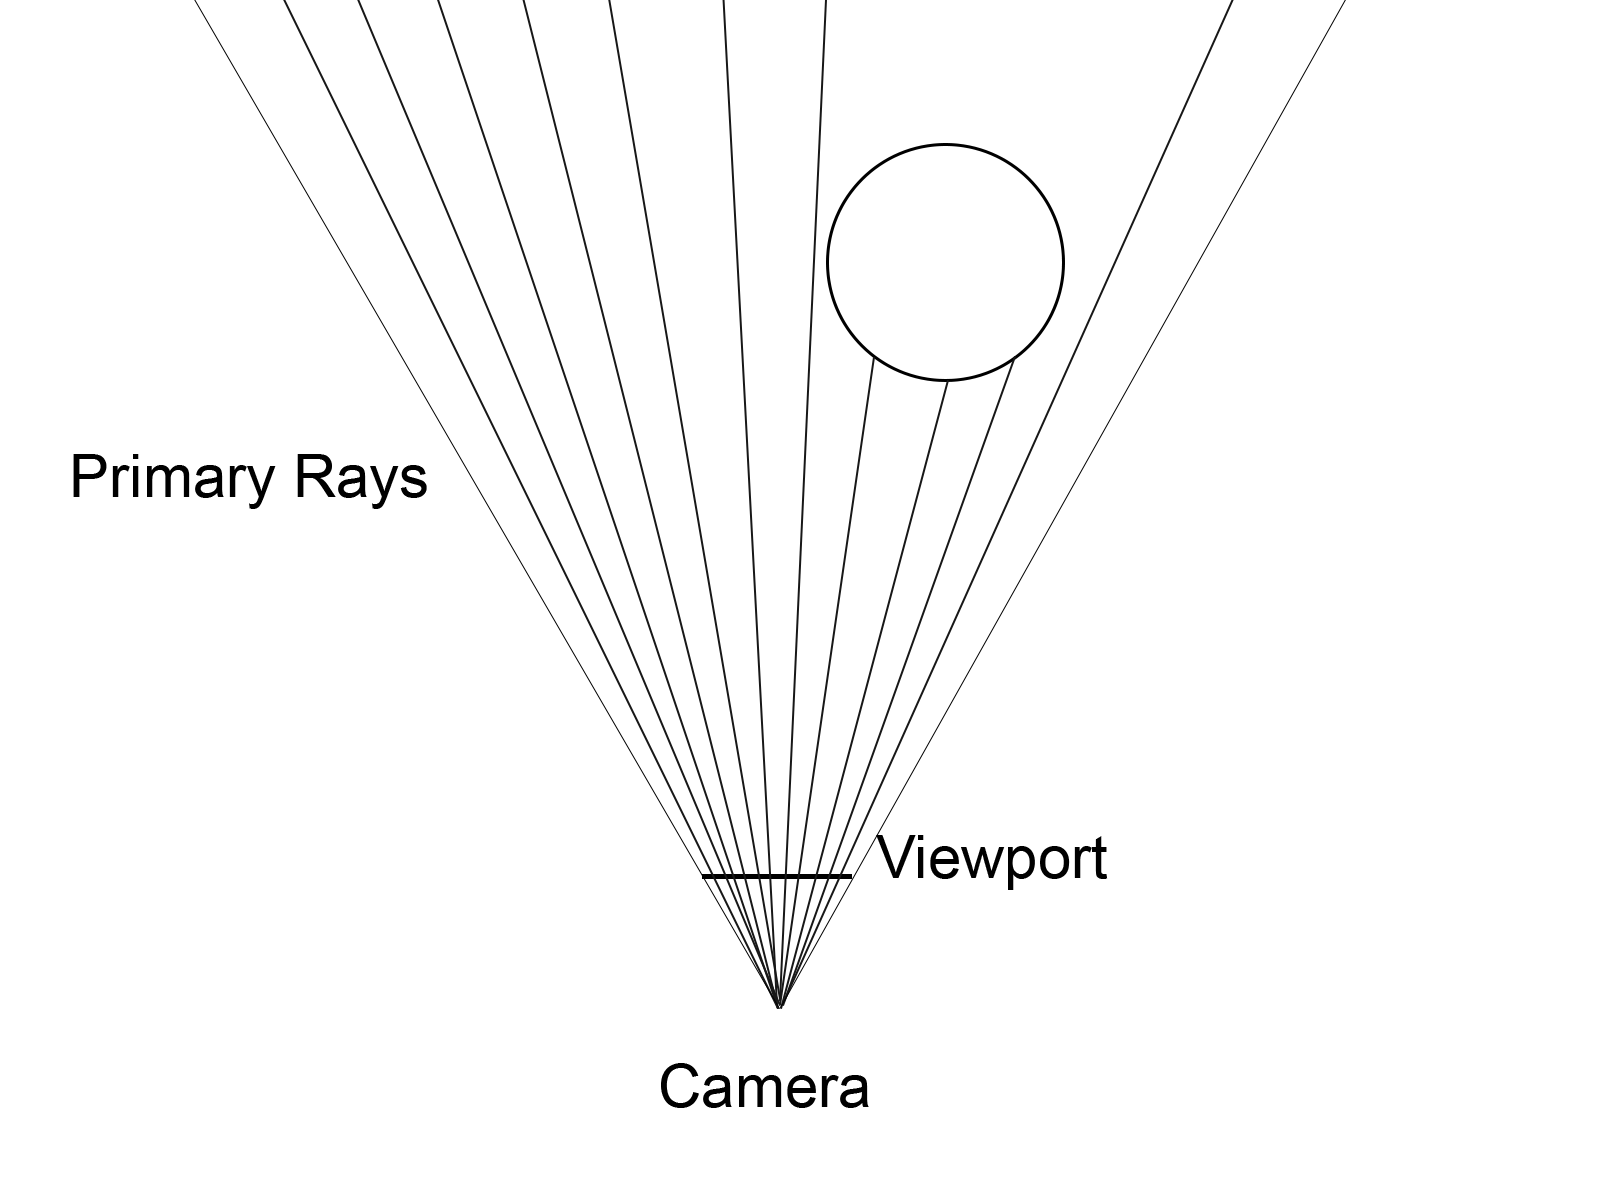
\includegraphics[width=14cm]{primaryray.png}
	\caption{Primary rays being cast into the scene to determine intersection with the sphere. A primary ray is spawned for every pixel in the viewport}
	\label{fig:ray_casting}
\end{figure}

Once the primary ray has intersected the scene, secondary rays can be spawned to determine the contribution of light from reflection, refraction, and also to check whether the path to each light in the scene is occluded in order to determine the contribution of that light. By spawning these rays, ray tracing can easily produce realistic global reflection and refraction within the scene.

\begin{figure}
\centering
	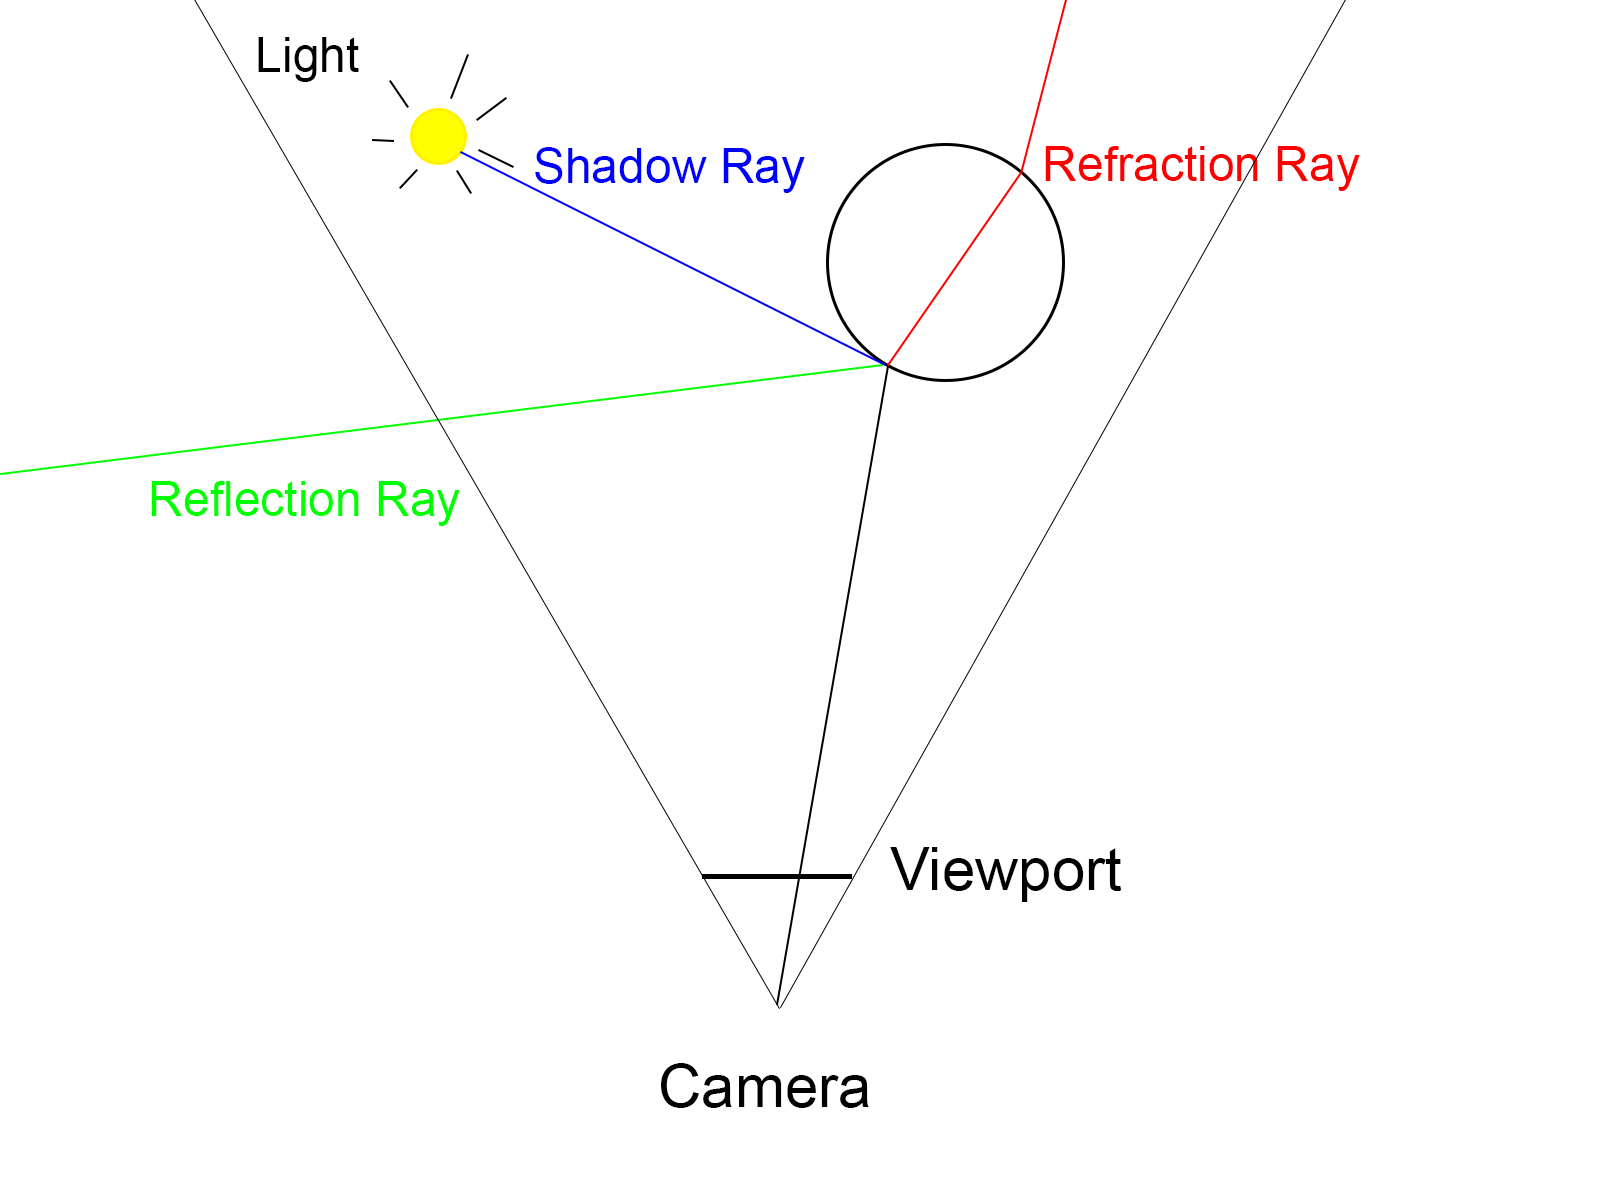
\includegraphics[width=14cm]{secondaryrays.png}
	\caption{Once primary intersection is determined, secondary rays can be spawned in order to determine reflection, refraction, and shadow coverage}
	\label{fig:ray_tracing}
\end{figure}

Another advantage of ray tracing over rasterisation is that it can be adapted to any data for which an intersection test with a ray can be devised. For example, the intersection of a ray with a volume stored within an array can be determined by stepping along the ray from the eye and stopping only when an intersection is detected or the volume is exited.

Once the ray-tracing algorithm has been adapted to consider the volumes, it is also possible to let it peer into volumes in order to consider the interior of the volume when calculating the colour of the final pixel on the screen. In this way, it is similar to the approach used in \cite{engel02interactivehigh-quality}, in that overlapping parts of the volume can be considered.

For example, as in figure \ref{fig:homogeneous_refraction}, a volume with a homogeneous index of refraction would be possible to consider by just considering the difference in index of refraction at the surfaces, and therefore would be possible to model using geometry alone.

\begin{figure}
\centering
	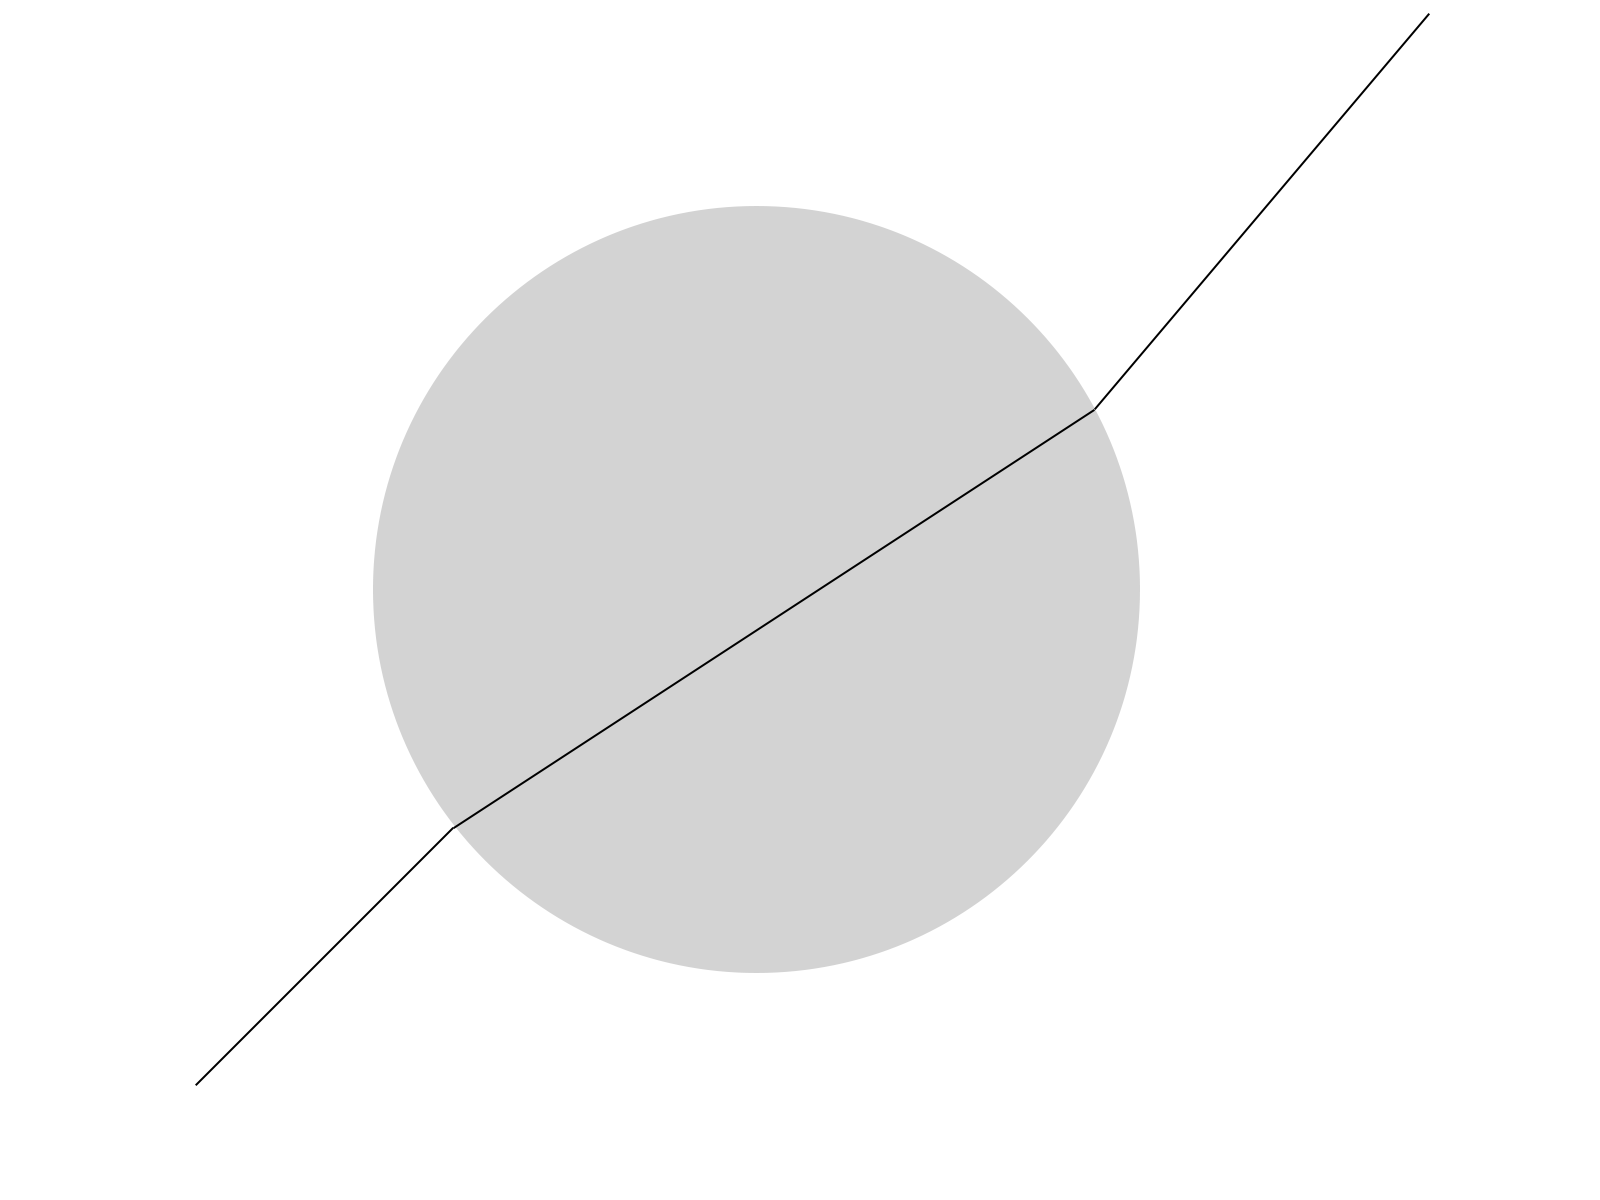
\includegraphics[width=12cm]{homogeneousrefraction.png}
	\caption{Ray traced refraction through a homogeneous volume}
	\label{fig:homogeneous_refraction}
\end{figure}

On the other hand, modelling refraction through a volume with a varying index of refraction, as in figure \ref{fig:heterogeneous_refraction}, this approach would quickly become infeasible for volumes of high heterogeneity. By allowing the ray tracing algorithm to consider the volume involved, rather than just the geometry, volumes high in heterogeneity can also be modelled, allowing complex visual effects to be simulated.

\begin{figure}
\centering
	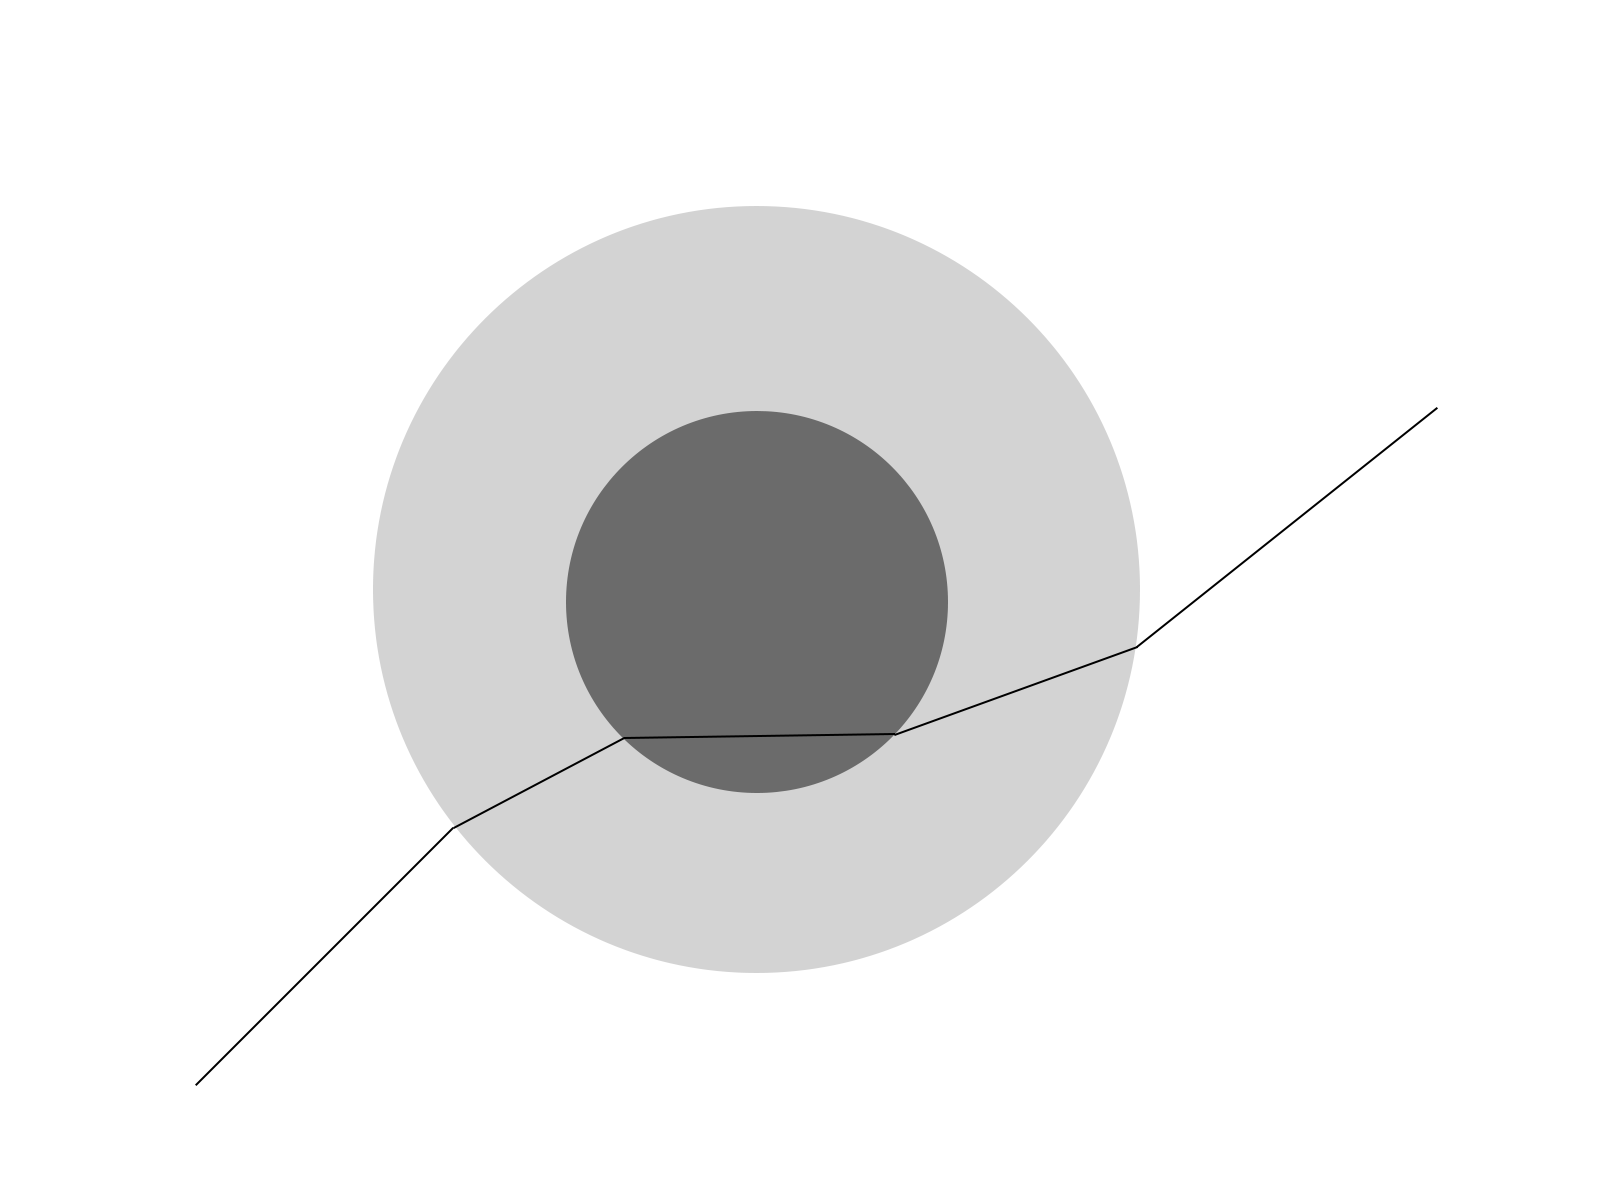
\includegraphics[width=12cm]{heterogeneousrefraction.png}
	\caption{Ray traced refraction through a heterogeneous volume}
	\label{fig:heterogeneous_refraction}
\end{figure}

In order to do this in real-time, however, it is necessary to parallelise this process in order to render at a reasonable resolution to allow image quality as high as that of rasterisation.

\section{General-purpose processing on the GPU}
Around the turn of the century, the traditional graphics pipeline became more flexible with the introduction of the programmable graphics pipeline. This has turned the GPU into a massively parallel SIMD (single instruction, multiple data) processor, capable of performing highly parallelised computation by running the same instructions on many pieces of data at once.

With the emergence of general purpose programming languages such as OpenCL and CUDA, the GPU has become a general purpose processing tool capable of processing any parallelisable algorithm extremely quickly, redefining the problem of volume rendering on the GPU from mapping volume rendering problems to fixed rasterisation operations, to the utilisation of the GPU's massively parallelisable SIMD computation model.

It turns out that ray tracing maps very favourably to this model, as each ray must do roughly the same computation, but with different input data. By processing these rays on the GPU, for example, every pixel of the screen could be considered in parallel, allowing high screen resolutions to be considered without greatly increasing the time of computation.

\section{Storage}
Another challenging problem in volume rendering is representing true heterogeneous volumes. Naive volume storage approaches using arrays typically store data at a fixed resolution. The problem with this approach is that, in order to store any of the volume at a high enough resolution to represent it accurately, the whole volume must be stored at that resolution. For complex scenes, this can very quickly become prohibitively expensive.

In addition, it is also unnecessary. Large regions of the scene may be empty, homogeneous, or identical to other regions. With such an approach, these regions have exactly the same memory footprint as any other identically-sized region of the volume.

Ideally, we should be able to store any volume at a high enough resolution such that it can be represented accurately, without any unwanted visual artifacts. Numerous researchers have suggested approaches that avoid this problem by using hierarchical data structures.

\subsection{Hierarchical data structures}
Hierarchical, or tree, data structures, are structures for representing 3D volumes that start by encoding data at a low resolution, covering large areas of the volume, and becoming higher resolution the deeper one traverses into the hierarchy. Once the encoded region is a sufficiently good approximation of the original volume, the hierarchy does not need to go any lower.

\begin{figure}
\centering
	\centering
	\subfloat[]{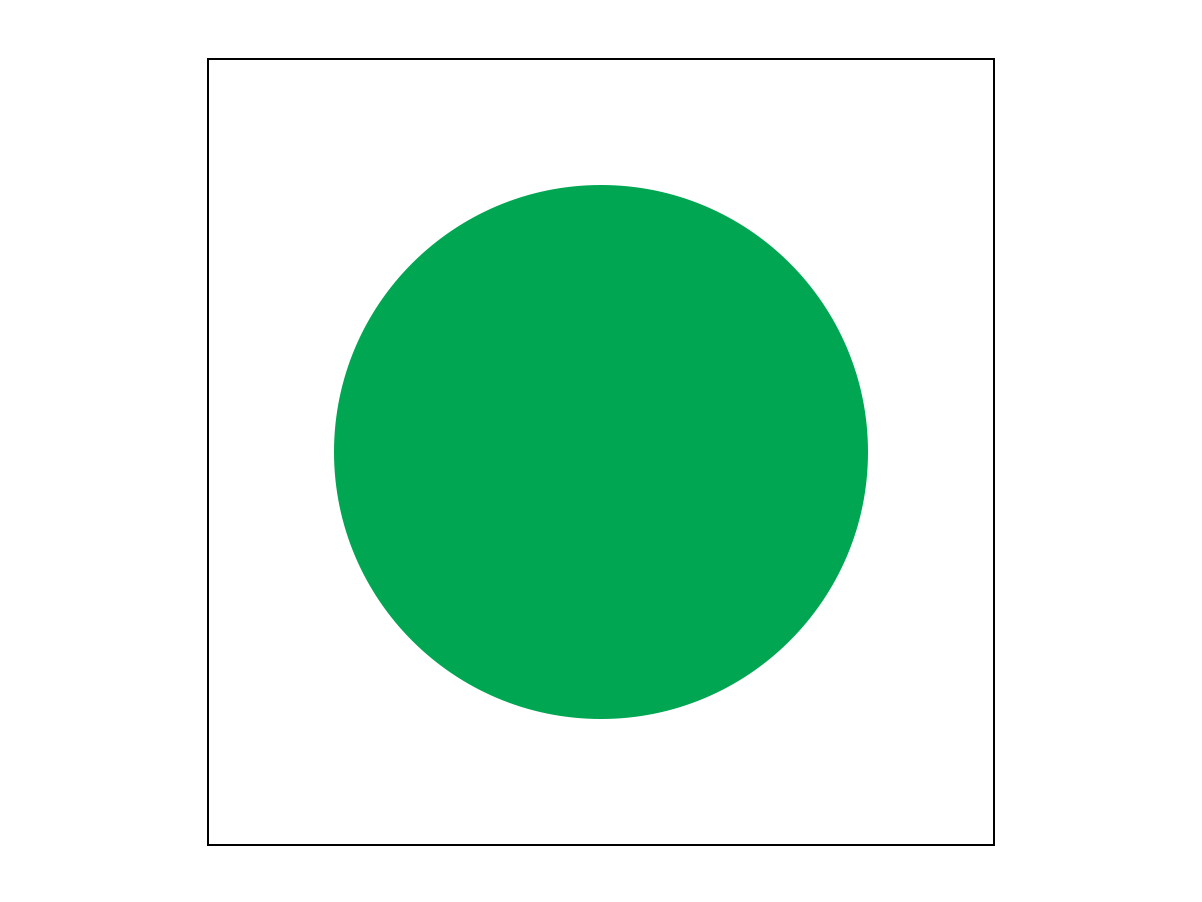
\includegraphics[width=3in]{tree_root.png}}
	~
	\subfloat[]{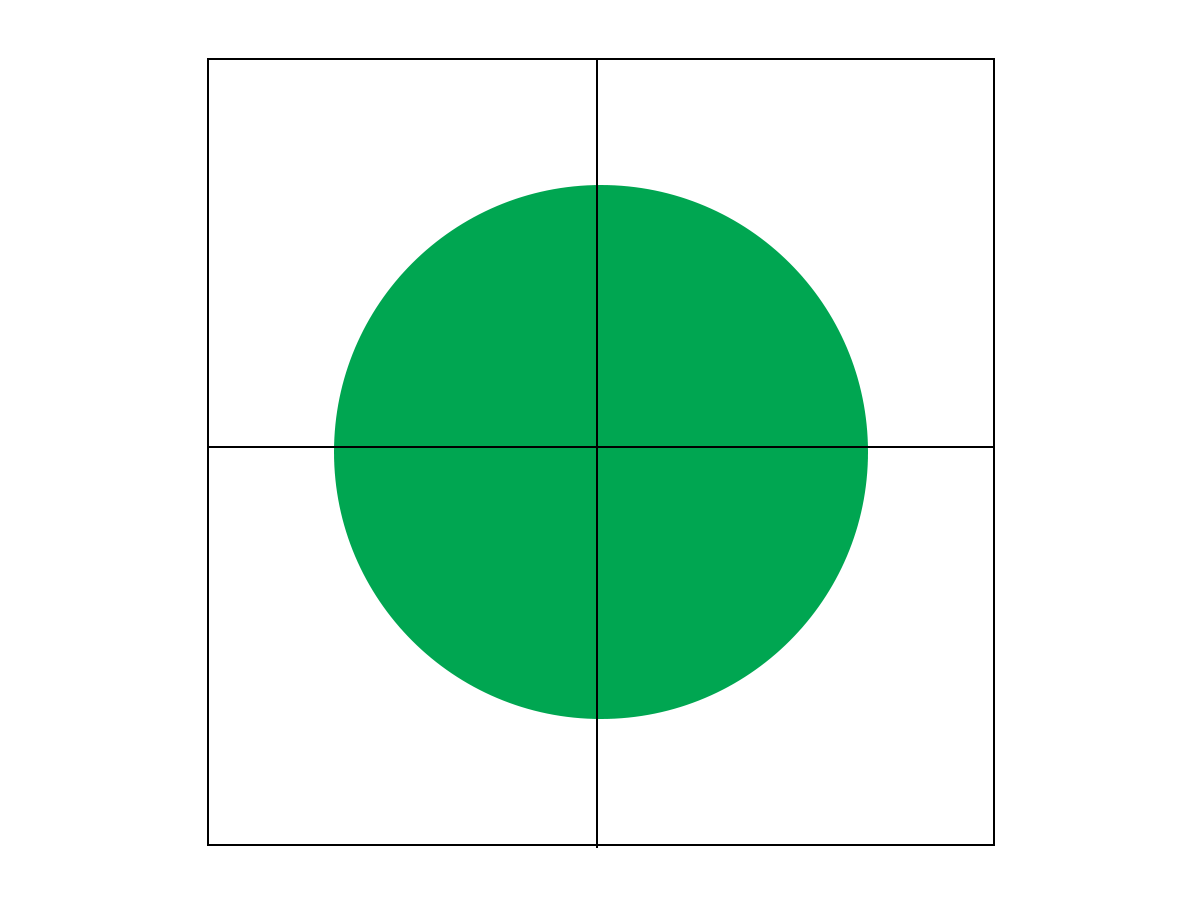
\includegraphics[width=3in]{tree_level1.png}}
	\\
	\subfloat[]{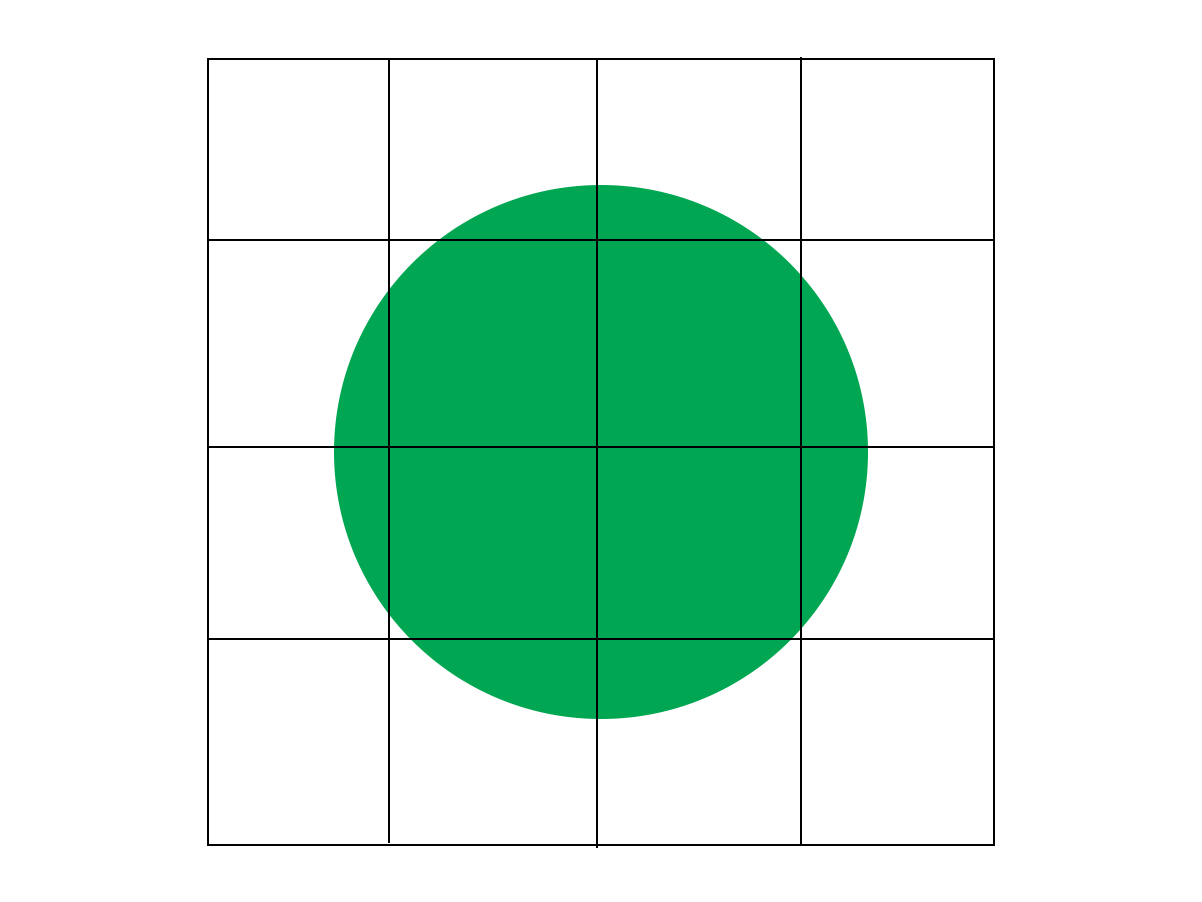
\includegraphics[width=3in]{tree_level2.png}}
	~
	\subfloat[]{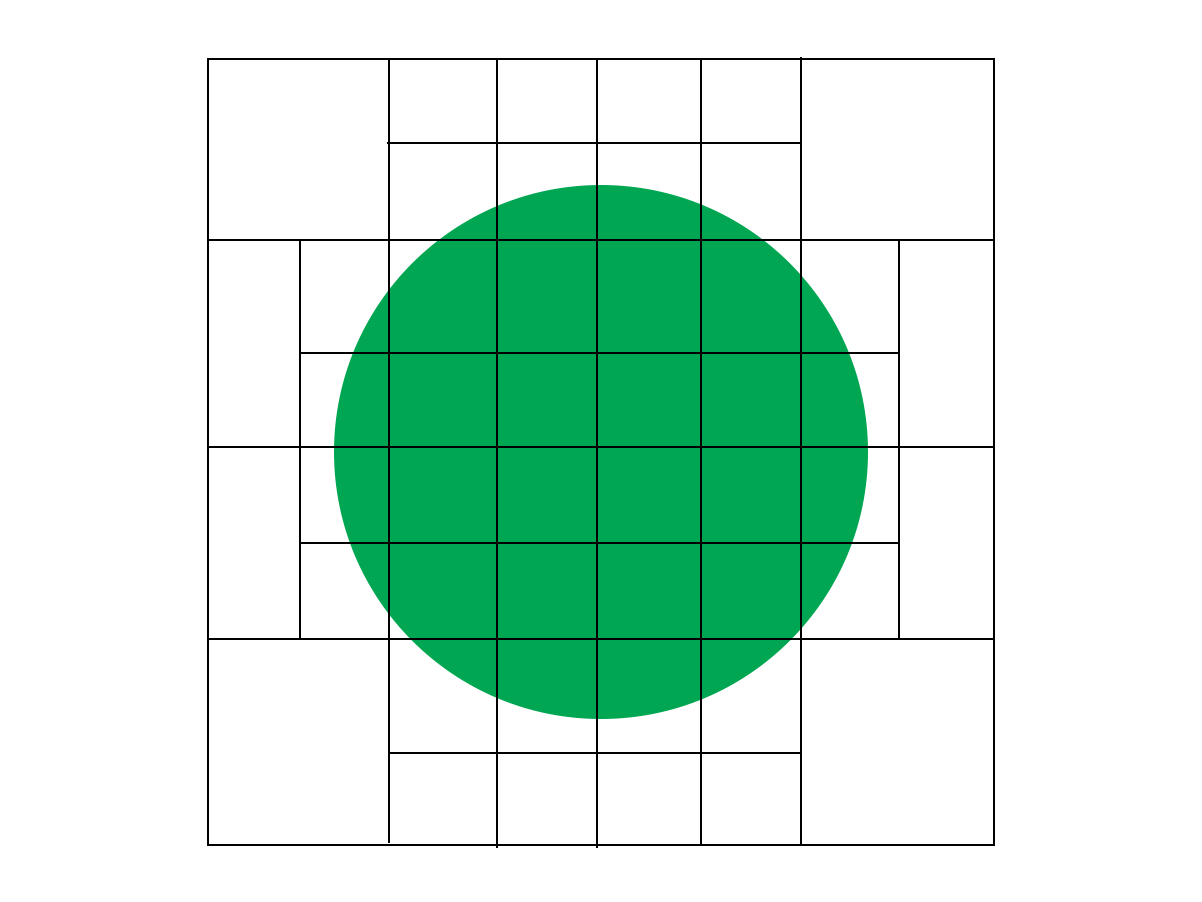
\includegraphics[width=3in]{tree_level3.png}}

	\caption{The construction of a hierarchical volume representation. As demonstrated by (d), empty nodes are not divided further}
	\label{fig:space_subdivision}
\end{figure}

An additional advantage of this type of structure is that one does not need to encode areas of empty space, and during traversal, large areas of empty space can be skipped at the more coarse levels of the hierarchy. The construction of such a structure has been demonstrated in figure \ref{fig:space_subdivision}.

\begin{figure}
\centering
	\subfloat[]{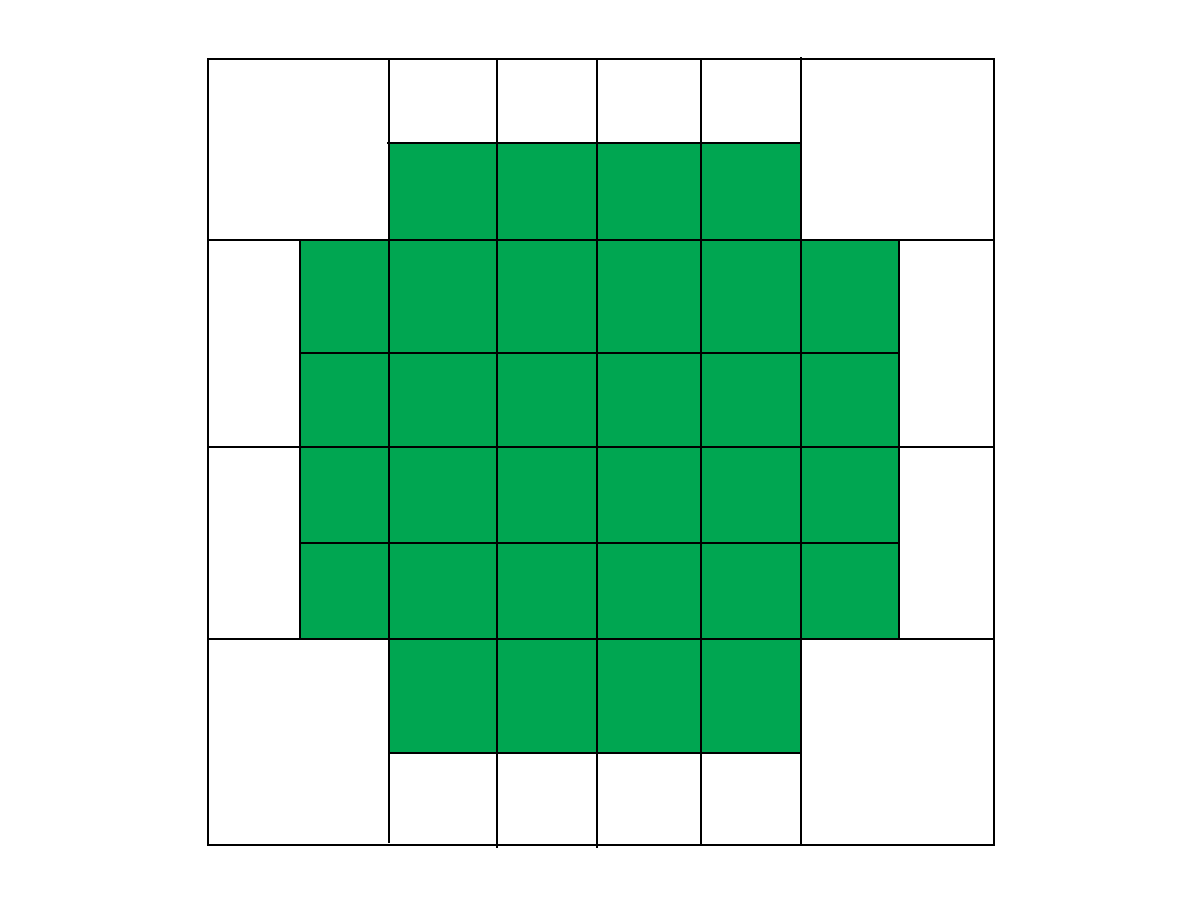
\includegraphics[width=3in]{3level_leaves.png}}
	~
	\subfloat[]{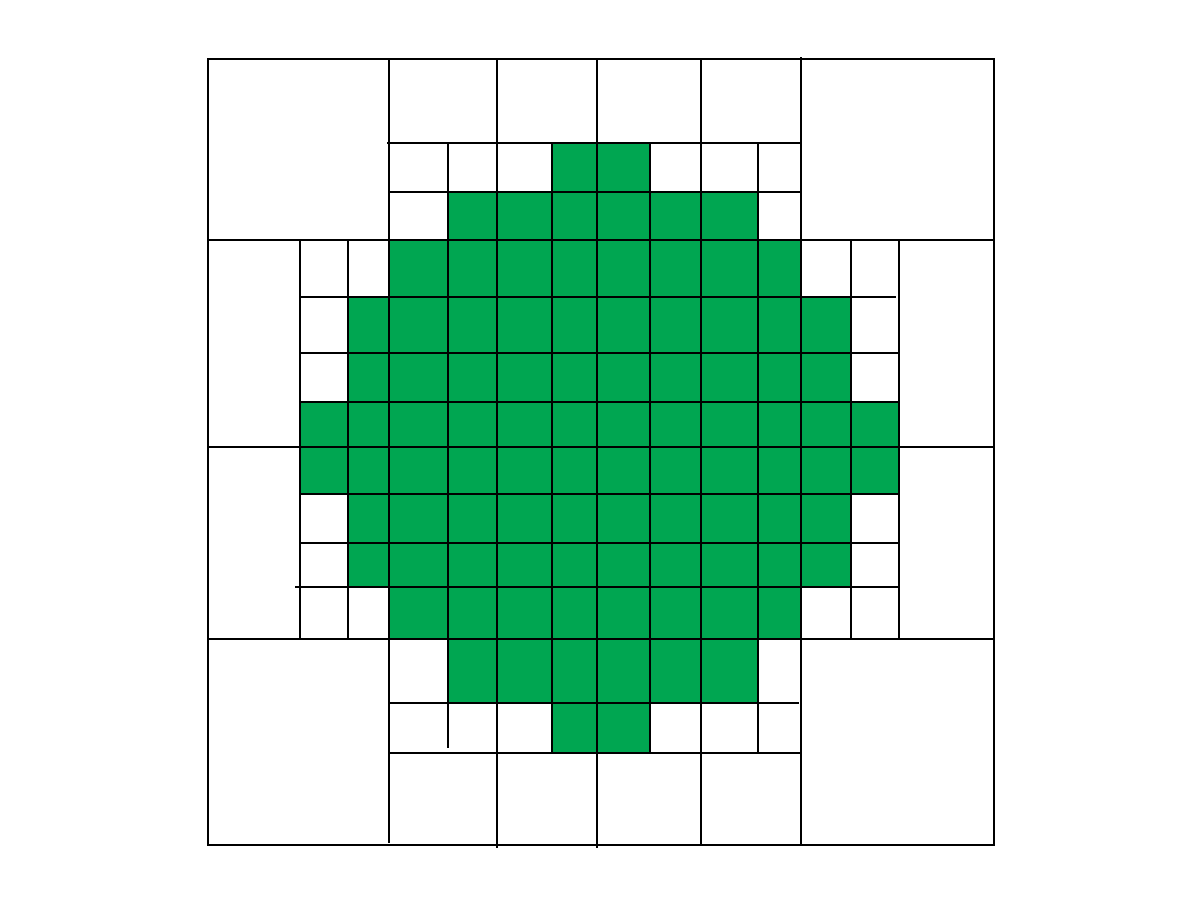
\includegraphics[width=3in]{4level_leaves.png}}

	\caption{Rendering the leaves of the tree results in an approximation of the volume. As the number of subdivisions is increased, the approximation improves}
	\label{fig:tree_leaves}
\end{figure}

\section{Objectives}

Our primary objective is to develop a renderer that can simulate true volumetric effects by means of ray tracing. This renderer should be able to handle heterogeneous volumes as well as homogeneous volumes, taking into account global effects, where the rest of the scene can affect the rendering of any one part.

In addition, this renderer should be able to function with real-time performance on ubiquitous consumer-level graphics hardware. To accomplish this, we intend to utilise general purpose GPU programming and develop a highly parallelisable method of rendering that utilises the SIMD nature of graphics hardware.

Our renderer also needs to support a compact volume format which is capable of representing highly heterogeneous regions as well as homogeneous regions, with a small enough memory footprint to fit in GPU memory. In order to accomplish this we intend to take advantage of hierarchical data structures which allow us to store volumes of varying resolution and avoid storing empty space.